\documentclass[UTF8]{ctexbeamer}
\usefonttheme{serif}
\usepackage[labelformat=empty]{caption}

% 设置主题
\usetheme{Berkeley}

% 标题、作者、日期等
\title{Seperation of the Water Columns in Water Hammer Event}
\author{刘锦坤;姜逸轩;黑建聪}
\date{\today}

% 开始文档
\begin{document}

% 标题页
\begin{frame}
    \titlepage
\end{frame}

% 目录页
\begin{frame}{Outline}
    \tableofcontents
\end{frame}

% Water Hammer Event
\section{Water Hammer Event}
\begin{frame}{Water Hammer Event}
    A water hammer is a type of wave that generates shock waves due to the inertia of the pressure water flow during sudden power outages or when the valve is closed too quickly, just like a hammer striking. The force generated by the back and forth flow of water shock waves can sometimes be significant, causing damage to valves and pumps.
\end{frame}

% Column Seperation
\section{Column Seperation}
\begin{frame}{Column Seperation}
    Column separation refers to the breaking of liquid columns in fully filled pipelines. This may occur in a water-hammer event when the pressure in a pipeline drops to the vapor pressure at specific locations such as closed ends, high points or knees (changes in pipe slope). The liquid columns are separated by a vapor cavity that grows and diminishes according to the dynamics of the system. The collision of two liquid columns, or of one liquid column with a closed end, may cause a large and nearly instantaneous rise in pressure. This pressure rise travels through the entire pipeline and forms a severe load for hydraulic machinery, individual pipes and supporting structures. The situation is even worse: in one water-hammer event many repetitions of cavity formation and collapse may occur.
    
    \textbf{So we need a theoretical numerical way to calculate the state parameters as an analytical method!}
\end{frame}

% Water Hammer Event Calculation without Considering Seperation
\section{Water Hammer Event Calculation without Considering Seperation}
\begin{frame}{Water Hammer Event Calculation without Considering Seperation}
    An common method is MOC (method of characteristics), which is literally the first assignment of the course and is familiar to all of us. Don't bother to repeat.
    
    \textbf{But there do exist problems:}
    \begin{itemize}
        \item Pressure drops significantly below the vapor pressure. According to thermodynamic theory, can't this happen!
        \item So vapor cavity would be generated, and therefore diminish, causing significantly dynamic effects.
    \end{itemize}
\end{frame}

% A Simple Way To Calculate The Seperation Effect
\section{A Simple Way To Calculate The Seperation Effect}
\begin{frame}{A Simple Way To Calculate The Seperation Effect}
    According to the artificial context, a commonly used way is called \textbf{The discrete vapor cavity model (DVCM)}, which can be demonstrated as the figure shown below:
    
    \begin{figure}
        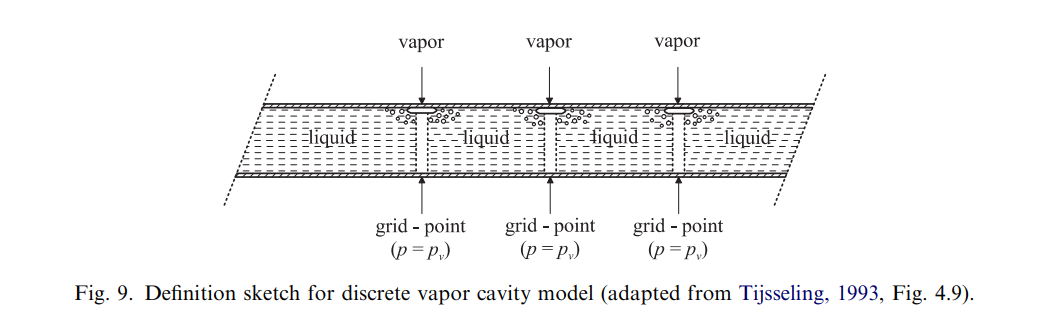
\includegraphics[width=0.7\textwidth]{image.png}
        \caption{Schematic Figure}
    \end{figure}
\end{frame}
    
\begin{frame}{A Simple Way To Calculate The Seperation Effect}
    Cavities are allowed to form at any of the computational sections (grid points) if the pressure is computed to be below the vapor pressure. Vapor cavities are thus confined to computational sections as sketched in Fig above and pure liquid with a constant pressure wave speed is assumed in between. The absolute pressure in a cavity is set equal to the vapor pressure:
    \begin{equation}
        p = p_v
    \end{equation}
    and the upstream and downstream discharges $Q_{Pv}$ and ${Q_P}$ at a cavity are computed from the compatibility. The cavity volume $e$ follows then from
    \begin{equation}
        \dot e = Q_{P} - Q_{Pv}
    \end{equation}
\end{frame}

\begin{frame}{A Simple Way To Calculate The Seperation Effect}
    A discrete form
    $$ 
    e^{t+dt} -e^{t} =  (\psi (Q_P^{t+dt}-Q_{Pv}^{t+dt}) + (1-\psi) (Q_P^{t}-Q_{Pv}^{t}))\cdot dt
    $$
    notitcing that $\psi$ is hyper-parameter dependent on experiment, probabally a task of our group is to adjust the $\psi$ to gain good results.
\end{frame}

\begin{frame}{Now the Task}
    Establish the model on python or MATLAB, verify the effectiveness of the DVCM and attempt to explain some physical features.
\end{frame}

\begin{frame}{Future the Work}
Apparently, the DVCM is not an complete model, it is also our goal to establish other models, including high-dimentional models (not 1-dimentional trivial model), such as shadow-flow model, 2-phase flow model, etc. CFD simulation may be considered, too.
\end{frame}

\end{document}